\subsection{Fortran IR (FIR)}

The LLVM Fortran frontend ``flang'' is currently under major development,
led by NVIDIA/PGI. Similar to Swift, Rust, and others, flang needs
a specialized IR in order to support advanced transformations
for high-performance Fortran codebase, and is using \MLIR to support
these Fortran-specific optimizations~\cite{flang}.  These high-level
optimizations---advanced loop
optimizations, array copy elimination, call specialization,
devirtualization---would be hard implement using only LLVM.

For example, FIR is able to model Fortran virtual dispatch table as a first
class concept (see~\figref{fir}).

\begin{figure}[h]
  \centering
  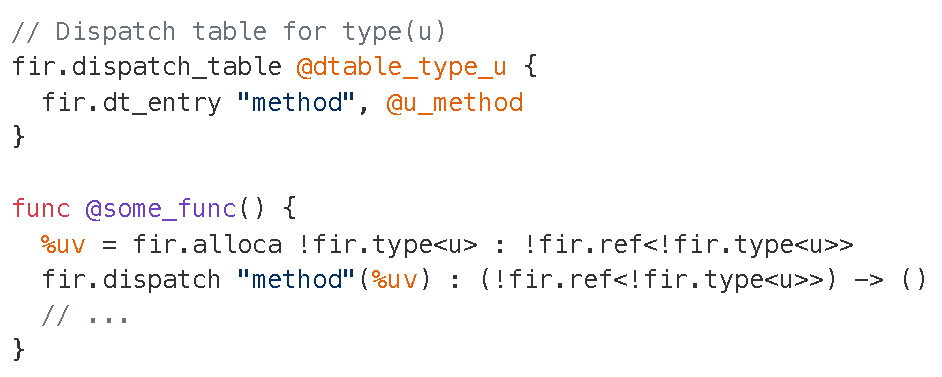
\includegraphics[width=.7\textwidth]{img/flang_mlir.pdf}
%\begin{tabular}{c}
%\begin{lstlisting}[language=mlir]
%// Dispatch table for type(u)
%fir.dispatch_table @dtable_type_u {
%  fir.dt_entry "method", @u_method
%}
%
%func @some_func() {
%  %uv = fir.alloca !fir.type<u> : !fir.ref<!fir.type<u>>
%  fir.dispatch "method"(%uv) : (!fir.ref<!fir.type<u>>) -> ()
%  // ...
%}
%\end{lstlisting}
%\end{tabular}

\caption{FIR has first class support for dynamic virtual function
dispatch table.}\label{fig:fir}
\end{figure}

The ability to model the high-level semantics of the programming language in a
structured IR is very powerful. For example, first-class modeling of the
dispatch tables allows a robust devirtualization pass to be implemented.  While
this could have been implemented with a bespoke compiler IR, the
use of \MLIR allowed the flang developers to spend their engineering resources
focused on the IR design for their domain instead of reimplementing basic
infrastructure.

The choice of \MLIR also unlocks the reusability of other dialects that are not
specific to Fortran: a language-independent OpenMP dialect could be shared
between Fortran and C language frontends.  Similarly, targeting a
heterogeneous platform using OpenACC
becomes tractable within \MLIR through the sharing and reuse of the
GPU-oriented dialects and passes. This is straightforward thanks to \MLIR 
begin specifically designed to support a mix of composable dialects.

